\section{Methods}

In the following, we will use definitions and notations introduced by
\citet{rougier:2011} where a neural map is defined as the projection from a
manifold $\Omega \subset \mathbb{R}^d$ onto a set $\mathcal{N}$ of $n$ {\em
  neuron}s which is formally written as $\Phi : \Omega \rightarrow
\mathcal{N}$. Each neuron $i$ is associated with a code word $\mathbf{w}_i \in
\mathbb{R}^d$, all of which established the set $\{\mathbf{w}_i\}_{i \in
  \mathcal{N}}$ that is referred as the code book. The mapping from $\Omega$ to
$\mathcal{N}$ is a closest-neighbor winner-take-all rule such that any vector
$\mathbf{v} \in \Omega$ is mapped to a neuron $i$ with the code
$\mathbf{w}_\mathbf{v}$ being closest to the actual presented stimulus vector
$\mathbf{v}$,
\begin{equation}
\Phi : \mathbf{v} \mapsto argmin_{i \in \mathcal{N}} (\lVert \mathbf{v} -
\mathbf{w}_i \rVert).
\label{eq:psi}
\end{equation}
The neuron $\mathbf{w}_\mathbf{v}$ is named the best matching unit (BMU) and
the set $C_i = \{x \in \Omega | \Phi(x) = \mathbf{w}_i \}$ defines the {\em
  receptive field} of the neuron $i$.


\subsection{Spatial distribution} % \& Centroidal Voronoi Tesselation}

The SOM space is usually defined as a two-dimensional region where nodes are
arranged in a regular lattice (rectangular or hexagonal). Here, we consider
instead the random placement of neurons with a specific spectral distribution
(blue). As explained by \citet{Zhou:2012}, the spectral distribution
property of noise patterns is often described in terms of the Fourier spectrum
color. White noise corresponds to a flat spectrum with equal energy distributed
in all frequency bands while blue noise has weak low-frequency energy, but
strong high-frequency energy. Said differently, blue noise has intuitively
good properties with points evenly spread without visible structure (see
figure~\ref{fig:sampling} for a comparison of spatial distributions).
%%
\begin{figure}[htbp]
  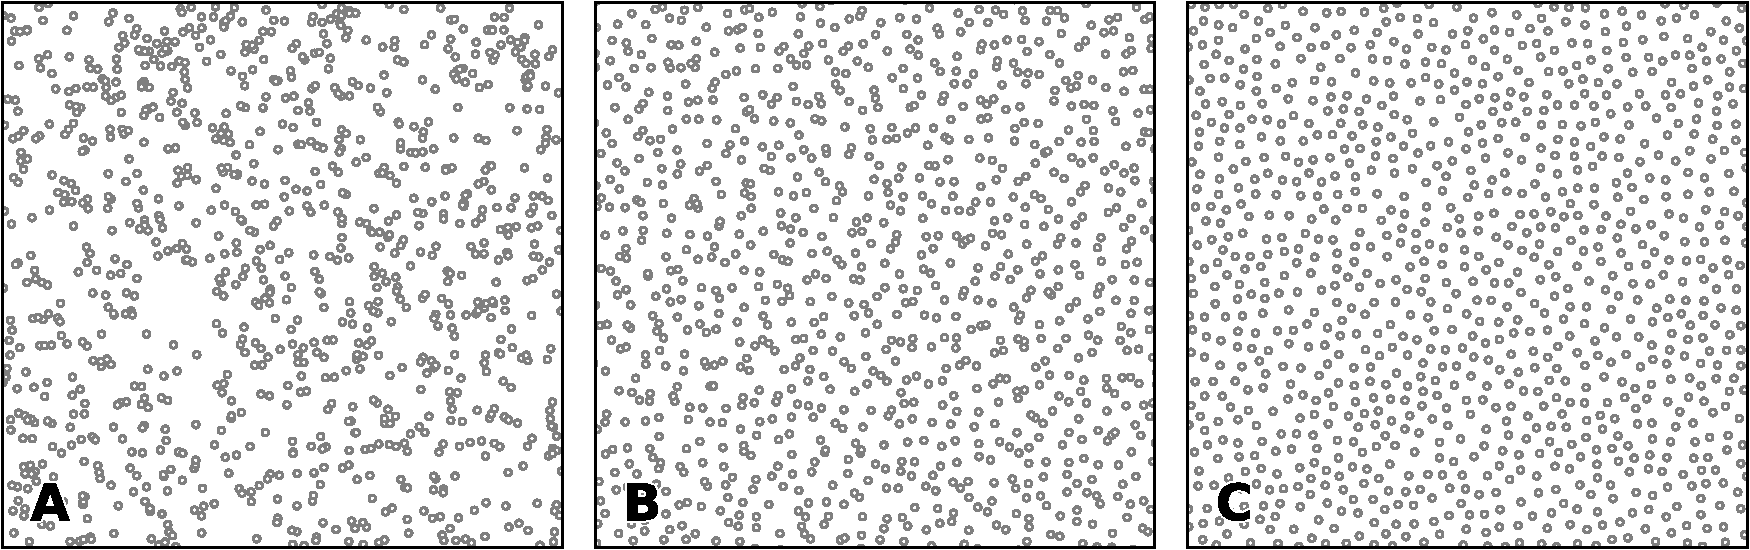
\includegraphics[width=\textwidth]{figures/blue-noise.pdf}
  \caption{\textbf{Spatial distributions.}
    \textbf{\textsf{A.}} Uniform sampling (n=1000) corresponding to white noise.
    \textbf{\textsf{B.}} Regular grid (n=32$\times$32) + jitter (2.5\%).
    \textbf{\textsf{C.}} Poisson disc sampling (n=988) corresponding to blue noise.}
  \label{fig:sampling}
\end{figure}
%%
There exists several methods \citep{Lagae:2008} to obtain blue noise
sampling that have been originally designed for computer graphics (e.g. Poisson
disk sampling, dart throwing, relaxation, tiling, etc.). Among these methods,
the fast Poisson disk sampling in arbitrary dimensions \citep{Bridson:2007}
is among the fastest (O(n)) and easiest to use. This is the one we retained for
the placement of neurons over a normalized $[0,1]\times[0,1]$ region. Such
Poisson disk sampling guarantees that samples are no closer to each other than
a specified minimum radius. This initial placement is further refined by
applying a LLoyd relaxation \citep{Lloyd:1982} scheme for 10 iterations,
achieving a quasi centroidal Voronoi tesselation.

\subsection{Topology}

Considering a set of $n$ points $P = \{P_i\}_{i \in [1,n]}$ on a finite region,
we first compute the Euclidean distance matrix $E = \{E_{ij}\}_{i,j \in [1,n]}
= \lVert P_i - P_j \rVert$ and we subsequently define a connectivity matrix
$G^{p} = \{G^{p}_{ij}\}_{i,j \in [1,n]}$ such that only the $p$ closest points
are connected. More precisely, if $P_j$ is among the $p$ closest neighbours of
$P_i$ then $G^p_{ij} = 1$ else we have $G^p_{ij} = 0$. From this connectivity
matrix representing a graph, we compute the length of the shortest path between
each pair of nodes and stored them into a distance matrix $D^p$. Note that
lengths are measured in the number of nodes between two nodes such that two
nearby points (relatively to the Euclidean distance) may have a correspoding
long graph distance as illustrated on figure \ref{fig:topology}. This matrix
distance is then normalized by dividing it by the maximum distance between two
nodes. In the singular case when two nodes cannot be connected through the
graph, we recompute a spatial distribution until all nodes can be connected.
%%
\begin{figure}
  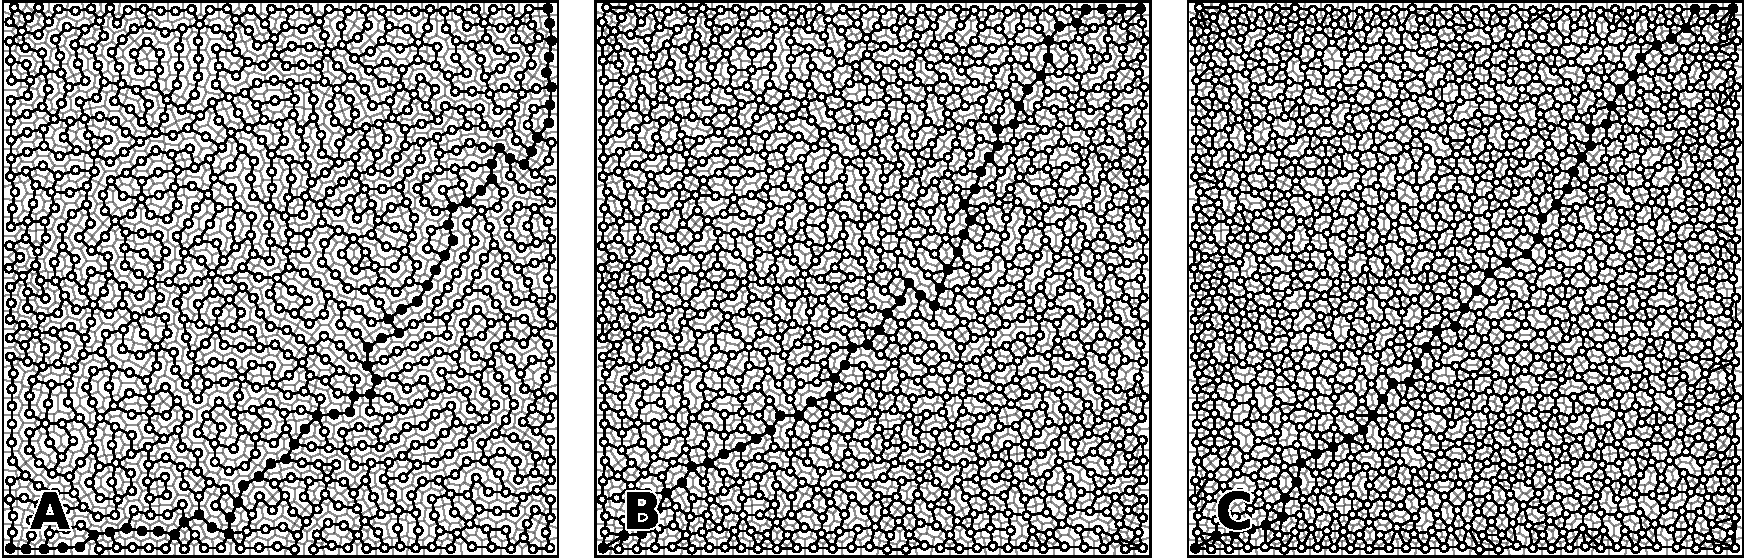
\includegraphics[width=\columnwidth]{figures/distances.pdf}
  \caption{\textbf{Influence of the number of neighbours on the graph
    distance.} The same initial set of 1003 neurons has been equiped with
    2-nearest neighbors, 3 nearest neighbors and 4-nearest neighbors induced
    topology (panels \textbf{A}, \textbf{B} and \textbf{C} respectively). A
    sample path from the the lower-left neuron to the upper-right neuron has
    been highlighted with a thick line (with respective lengths of 59, 50 and
    46 nodes).}
  \label{fig:topology}
\end{figure}


\subsection{Learning}

The learning process is an iterative process between time $t=0$ and time
$t=t_f \in \mathbb{N}^+$ where vectors $\mathbf{v} \in \Omega$ are sequentially
presented to the map with respect to the probability density function $f$. For
each presented vector $\mathbf{v}$ at time $t$, a winner $s \in \mathcal{N}$ is
determined according to equation (\ref{eq:psi}). All codes $\mathbf{w}_{i}$
from the code book are shifted towards $\mathbf{v}$ according to
\begin{equation}
  \Delta\mathbf{w}_{i} = \varepsilon(t)~h_\sigma(t,i,s)~(\mathbf{v} -
  \mathbf{w}_i)
  \label{eq:som-learning}
\end{equation}
with $h_\sigma(t,i,j)$ being a neighborhood function of the form
\begin{equation}
  h_\sigma(t,i,j) = e^{- \frac{{D^p_{ij}}^2}{\sigma(t)^2}}
  \label{eq:som-neighborhood}
\end{equation}
where $\varepsilon(t) \in \mathbb{R}$ is the learning rate and $\sigma(t) \in \mathbb{R}$
is the width of the neighborhood defined as
\begin{equation}
  \sigma(t) =
  \sigma_i\left(\frac{\sigma_f}{\sigma_i}\right)^{t/t_f}, \text{ with } \varepsilon(t) =
  \varepsilon_i\left(\frac{\varepsilon_f}{\varepsilon_i}\right)^{t/t_f},
\end{equation}
while $\sigma_i$ and $\sigma_f$ are respectively the initial and final
neighborhood width and $\varepsilon_i$ and $\varepsilon_f$ are respectively the
initial and final learning rate. We usually have $\sigma_f \ll \sigma_i$ and
$\varepsilon_f \ll \varepsilon_i$.


\subsection{Reorganization}

In case of neural loss (a set of neurons is removed from the map) or neural
gain (a set of neurons is added to the map), we can appy the LLoyd relaxation
scheme in order to achieve a new quasi centroidal Voronoi tesselation (see
figure \ref{fig:CVT}) whose induced topology shares similarity with the orginal
topology (before loss or gain).

\begin{figure}
  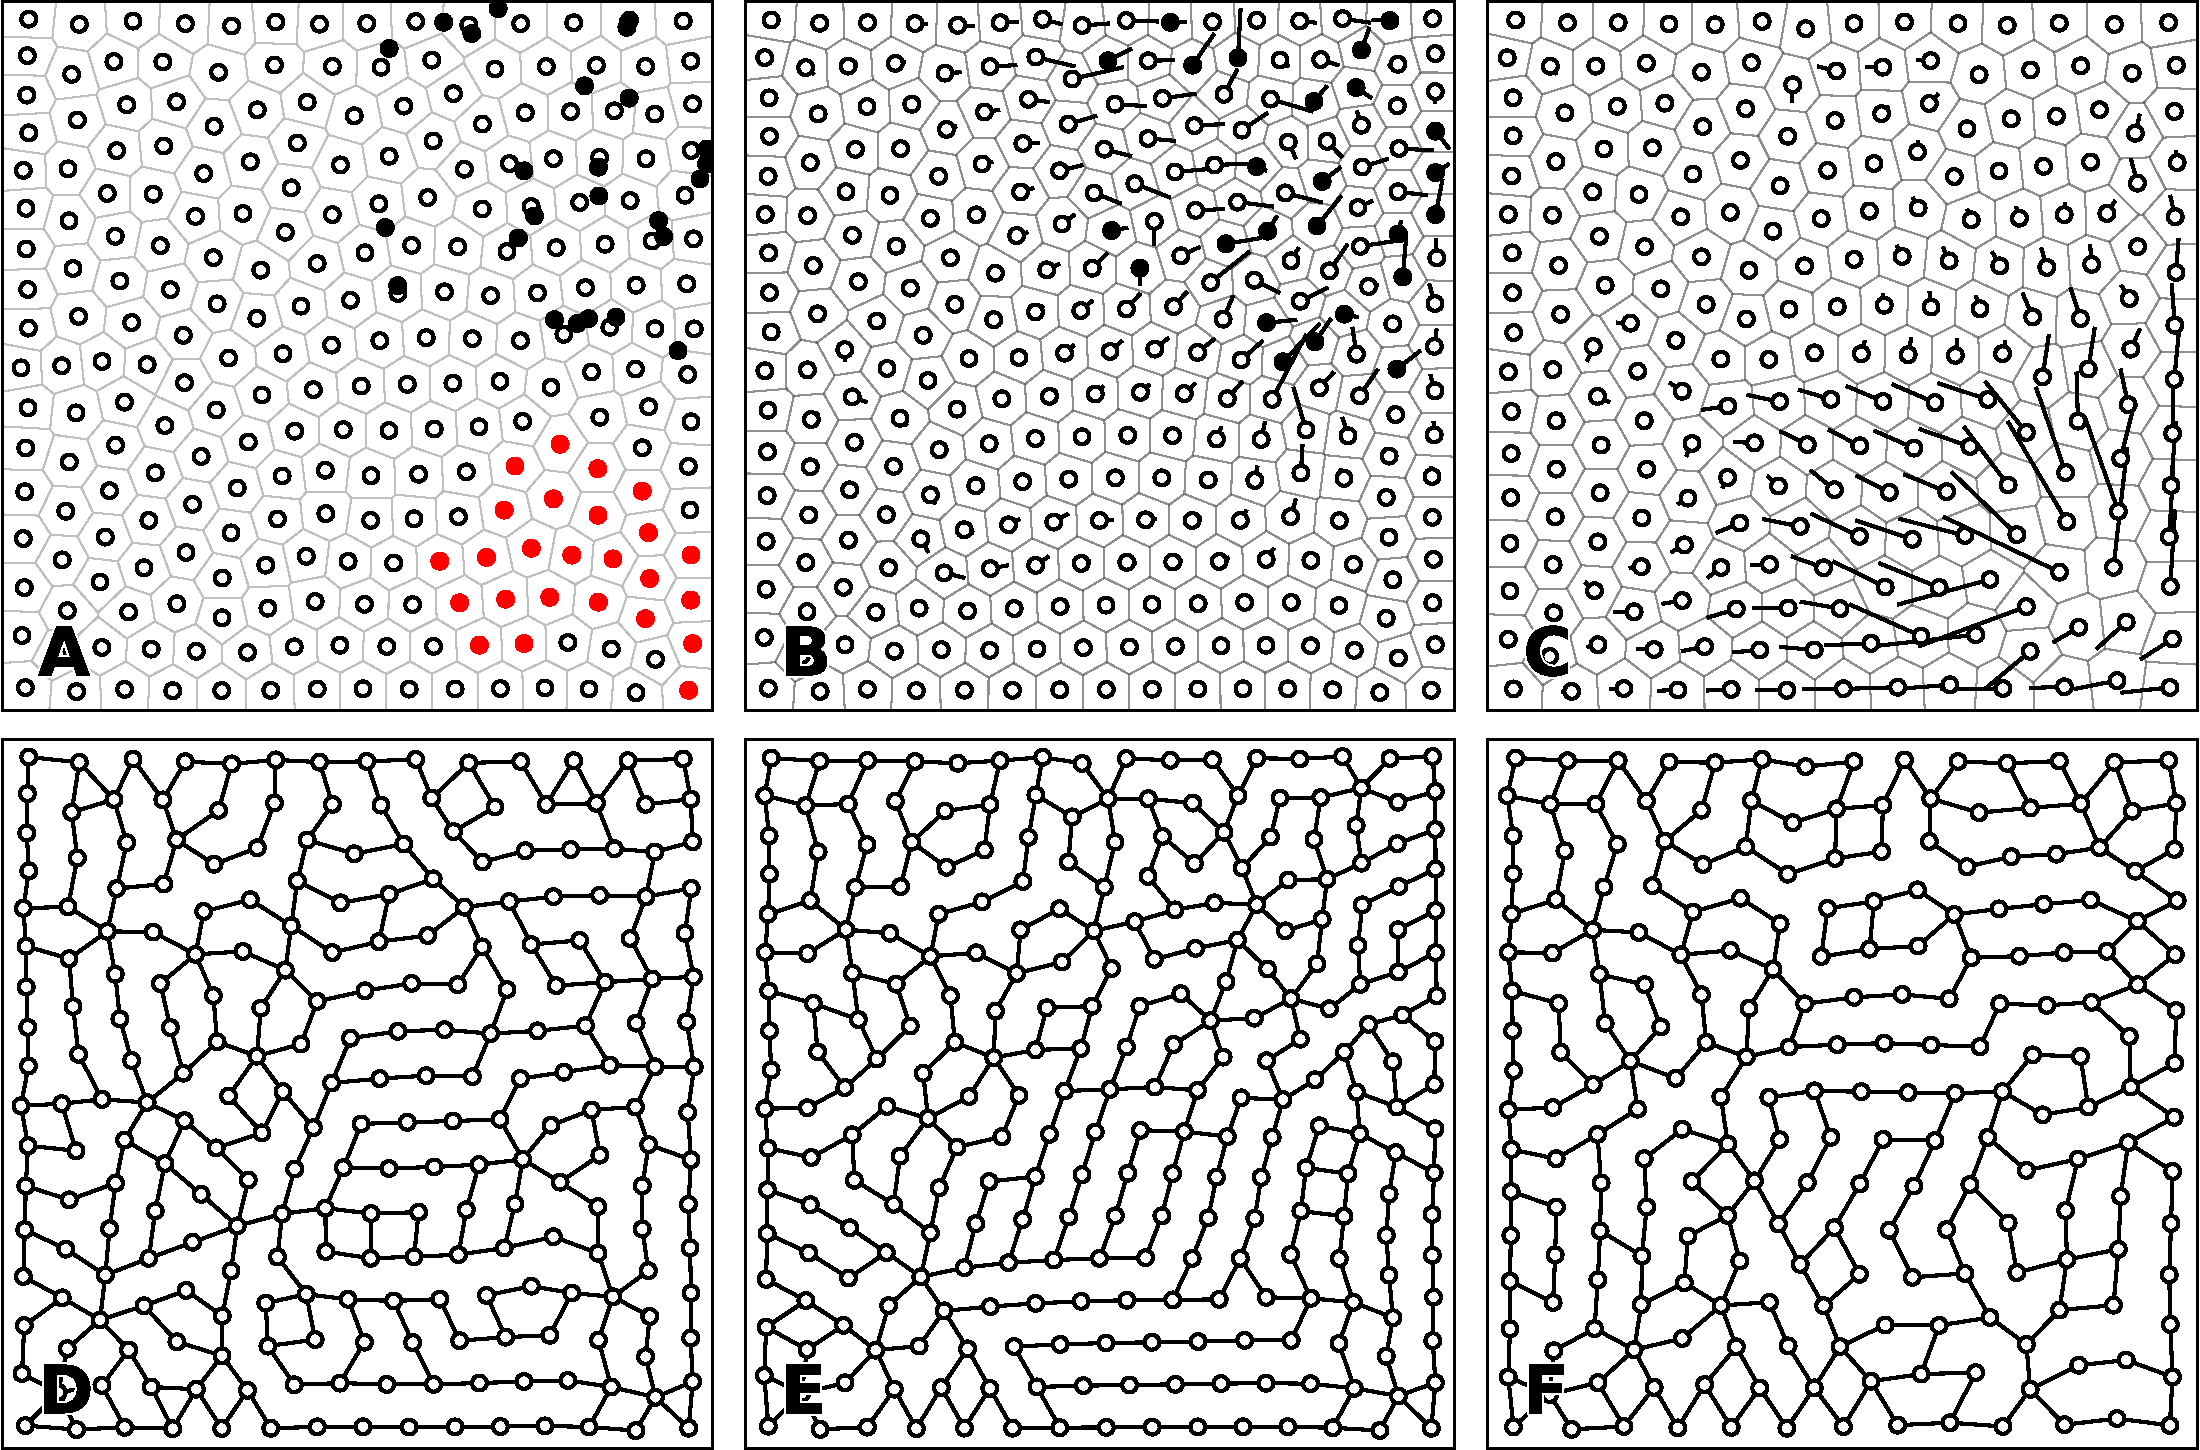
\includegraphics[width=\columnwidth]{figures/vsom-resilience.pdf}
  \caption{\textbf{Reorganization following neural loss or gain.}  An initial
    set of 248 neurons (outlined discs on panel \textbf{A}) has been modified
    with the addition of 25 neurons (black discs) or the removal of 25 neurons
    (red discs). Panels \textbf{B} and \textbf{C} show the final position of
    neurons after 100 iterations of the centroidal Voronoi tesselation. Lines
    shows individual movement of neurons. Panels \textbf{D}, \textbf{E} and
    \textbf{F} show the 2-neighbors induced topology for \textbf{A},
    \textbf{B} and \textbf{C} respectively.}
  \label{fig:CVT}
\end{figure}


%% Considering a set of $n$ points $P = \{P_i\}_{i \in [1,n]}$ on a finite domain
%% $D \in \mathbb{R}^2$, the Voronoi tesselation $V(P) = \{V_i\}_{i \in [1,n]}$ of
%% $P$ is defined as:
%% %
%% \begin{equation}
%%   \forall i \in [1,n], V_i = \{x \in D \mid
%%   \lVert x - P_i \rVert \leq \lVert x - P_j \rVert, \forall j \neq i\}
%% \end{equation}
%% %
%% Reciprocally, the (unique) Delaunay triangulation $T(P) = \{T_i\}_{i \in
%%   [1,n]}$ of $P$ is the dual graph of the Voronoi diagram and defined such that
%% no point in $P$ is inside the circumcircle of any triangles in $T(P)$. The
%% centers of the circumcircles are equivalent to the Voronoi diagram, i.e. a
%% partition of $D$ into Voronoi cells. For each of the cell $V_i$, we can compute
%% its centroid $C_i$ which is the center of mass of the cell. A Voronoi
%% tesselation is said to be centroidal when we have $\forall i \in [1,n], C_i =
%% P_i$ (see figure~\ref{fig:CVT}).\\

%% For an arbitrary set of points, there is no guarantee that the corresponding
%% Voronoi tesselation is centroidal but different methods can be used to
%% generate a centroidal tesselation from an arbitrary set of points. One of the
%% most straightforward and iterative methods is the Lloyd relaxation scheme
%% \citep{Lloyd:1982}:
%% \begin{enumerate}
%%   \item The Voronoi diagram of the $n$ points is computed
%%   \item The centroid of each of the $n$ Voronoi cell is computed.
%%   \item Each point is moved to the corresponding centroid of its Voronoi cell
%%   \item The method terminates if criterion is met (see below), else go to 1
%% \end{enumerate}
%% The algorithm finishes when the maximum distance between points and centroids
%% is less than a given threshold as illustrated in figure~\ref{fig:CVT}. It is
%% to be noted that because of numerical imprecisions, there is no guarantee that
%% an arbitrary small threshold can be reached.


%% \begin{figure}[htbp]
%%   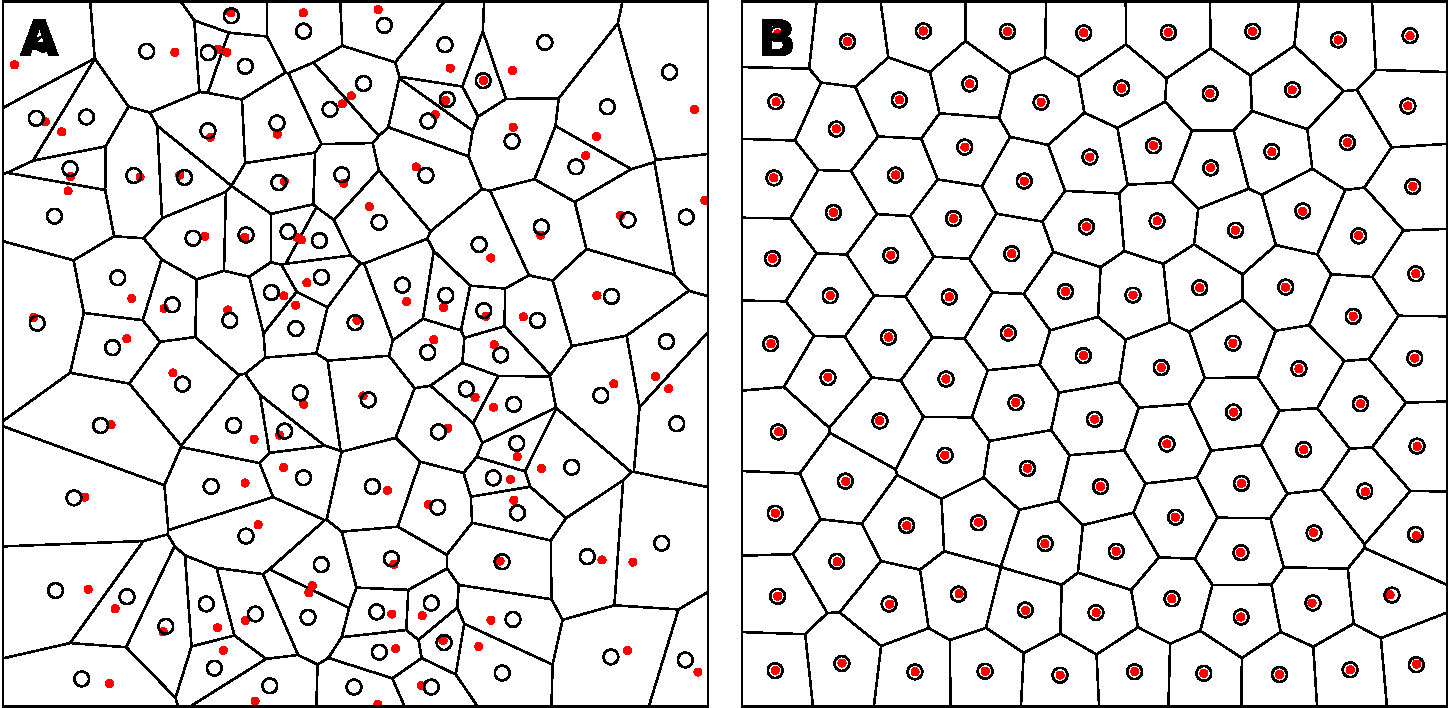
\includegraphics[width=\textwidth]{figures/CVT.pdf}
%%   \caption{\textbf{Centroidal Voronoi Tesselation.}  \textbf{\textsf{A.}}
%%     Voronoi diagram of a uniform distribution (n=100) where red dots represent
%%     the uniform distribution and white circles represent the centroids of each
%%     Voronoi cell. \textbf{\textsf{B.}} Centroidal Voronoi diagram where the
%%     point distribution matches the centroid distribution which constitutes a
%%     blue noise distribution (i.e. {\em a distribution that is roughly uniformly
%%       random with no preferred inter-point directions or distances} according
%%     to the definition of \citep{Ebeida:2014}). This figure has been obtained
%%     from the initial distribution on the left after 50 iterations of the Lloyd
%%     relaxation algorithm. }
%%   \label{fig:CVT}
%% \end{figure}
%
